\documentclass[smaller]{beamer}
%\VignetteIndexEntry{The R4X package}
%\SweaveOps{keep.source=T} 
\newcommand{\rfun}[1]{\texttt{#1}}


\usetheme{Goettingen}


\title{The R4X package}
\subtitle{Convenient XML manipulation for R}
\author{Romain Fran\c{c}ois}
\usebackgroundtemplate{
\includegraphics[width=\paperwidth]{pictures/gears-bright.jpg}}
\date{ version 0.1-17 of the package, 2008-06-27 }

\usepackage{/usr/local/lib/R/share/texmf/Sweave}
\begin{document}

{
 \usebackgroundtemplate{
\includegraphics[width=\paperwidth]{pictures/gears3.jpg}} 
 \setbeamertemplate{navigation symbols}{}
 \begin{frame}[fragile][plain]
\begin{center}

\begin{Huge}\textcolor{white}{\sf \bfseries The R4X package}\end{Huge}

\begin{Large}\textcolor{white}{\sf \bfseries Convenient XML Manipulation for R}\end{Large}
 
\end{center}

\begin{flushright}
 \begin{Large}
\textcolor{white}{\sf \bfseries Romain Fran\c{c}ois}  
 \end{Large}
\end{flushright}


 \end{frame}
}


\begin{frame}[fragile]
\frametitle{Outline}
\tableofcontents
\end{frame}

\section{Background}

\subsection{E4X}

\begin{frame}[fragile]
\frametitle{E4X}
\framesubtitle{Ecmascript (Javacript) for XML. Example from Wikipedia: \url{http://en.wikipedia.org/wiki/E4X} }

\begin{semiverbatim}
 var sales = <sales vendor="John">
    <item type="peas" price="4" quantity="6"/>
    <item type="carrot" price="3" quantity="10"/>
    <item type="chips" price="5" quantity="3"/>
  </sales>;
 
alert( sales.item.(@type == "carrot").@quantity );
alert( sales.@vendor );
for each( var price in sales..@price ) {
  alert( price );
}
\end{semiverbatim}
 
\end{frame}


\subsection{The XML package}           
 
\begin{frame}[fragile]
 \frametitle{The XML Package}
 \framesubtitle{from the $\hat{\Omega}$ project. \url{http://www.omegahat.org/RSXML/}}

This package provides facilities for the S language to

\begin{itemize}
    \item parse XML files, URLs and strings, using either the DOM (Document Object Model)/tree-based approach, or the event-driven SAX (Simple API for XML) mechanism;
    \item parse HTML documents,
    \item perform XPath queries on a document,
    \item generate XML content to buffers, files, URLs, and internal XML trees;
    \item read DTDs as S objects. 
\end{itemize}
\end{frame}

\begin{frame}[fragile]
 \frametitle{The XML Package in 3 slides}
 \framesubtitle{Creating XML content }

\begin{Schunk}
\begin{Sinput}
> x <- xmlNode( "test", 
     xmlNode( "bar", attrs = c( fruit = "mango") ), 
     xmlNode( "bar", attrs = c( fruit = "apple" )), 
   attrs = c(type="foo"))
> x
\end{Sinput}
\begin{Soutput}
<test type="foo">
 <bar fruit="mango"/>
 <bar fruit="apple"/>
</test>
\end{Soutput}
\begin{Sinput}
> class(x)
\end{Sinput}
\begin{Soutput}
[1] "XMLNode"
\end{Soutput}
\end{Schunk}

\end{frame}

\begin{frame}[fragile]
 \frametitle{The XML package in 3 slides}
\framesubtitle{Append content to an XML structure, the \rfun{addChildren} function}

\begin{Schunk}
\begin{Sinput}
> x
\end{Sinput}
\begin{Soutput}
<test type="foo">
 <bar fruit="mango"/>
 <bar fruit="apple"/>
</test>
\end{Soutput}
\begin{Sinput}
> addChildren( x, 
    xmlNode( "bar", attrs = 
      c( fruit = "pineapple" ) ) )
\end{Sinput}
\begin{Soutput}
<test type="foo">
 <bar fruit="mango"/>
 <bar fruit="apple"/>
 <bar fruit="pineapple"/>
</test>
\end{Soutput}
\end{Schunk}
\end{frame}


\begin{frame}[fragile]
 \frametitle{The XML package in 3 slides}
\framesubtitle{Query content of an XML structure}

\begin{Schunk}
\begin{Sinput}
> # The "fruit" attribute of the first child of x
> xmlAttrs( xmlChildren(x)[[1]], "fruit" )
\end{Sinput}
\begin{Soutput}
  fruit 
"mango" 
\end{Soutput}
\begin{Sinput}
> # The "fruit" attribute of each child of x
> xmlApply( x, xmlAttrs, "fruit" )
\end{Sinput}
\begin{Soutput}
$bar
  fruit 
"mango" 

$bar
  fruit 
"apple" 
\end{Soutput}
\end{Schunk}
\end{frame}



\section{Create XML}

\subsection{Create XML with R4X}
\begin{frame}[fragile]
\frametitle{The \rfun{xml} generic function}
\framesubtitle{The default method tries to convert strings into XML nodes, including nested nodes. Remember: Strings can be multiline in R.}
\begin{Schunk}
\begin{Sinput}
> y <- xml( '<test><foo blah="1"/><bar/></test>')
> y <- xml( '
    <test>
       <foo blah="1"/>
       <bar/>
    </test>
  ')
> y
\end{Sinput}
\begin{Soutput}
<test>
 <foo blah="1"/>
 <bar/>
</test>
\end{Soutput}
\begin{Sinput}
> class( y )
\end{Sinput}
\begin{Soutput}
[1] "XMLNode"
\end{Soutput}
\end{Schunk}
\end{frame}

\subsection{\texttt{brew}ing}
\begin{frame}[fragile]
\frametitle{Dynamic content with \rfun{brew}}
\framesubtitle{The \rfun{brew} package provides a psp-like templating framework for R. The \texttt{<\%=} operator is used by R4X to add dynamic content without
having to use \rfun{paste} or \rfun{sprintf}. } 
\begin{Schunk}
\begin{Sinput}
> f <- c("mango", "apple", "strawberry" )
> x <- xml( '
    <fruits>
      <fruit><%= f[1] %></fruit>
      <fruit><%= f[2] %></fruit>
      <fruit><%= f[3] %></fruit>
    </fruits>
  ')
> x 
\end{Sinput}
\begin{Soutput}
<fruits>
 <fruit>mango</fruit>
 <fruit>apple</fruit>
 <fruit>strawberry</fruit>
</fruits>
\end{Soutput}
\end{Schunk}
\end{frame}

\begin{frame}[fragile]
 \frametitle{More brewing}
\framesubtitle{The full rfun{brew} syntax can be used as well as just the \texttt{<\%=}, but it can become quickly difficult to manage. See the \rfun{distill}ing feature for stronger taste...}

\begin{Schunk}
\begin{Sinput}
> x <- xml( ' 
    <fruits>
      <%for( i in f) {%>
        <fruit><%= i %></fruit>
      <%}%>
    </fruits>
  ')
> x
\end{Sinput}
\begin{Soutput}
<fruits>
 <fruit>mango</fruit>
 <fruit>apple</fruit>
 <fruit>strawberry</fruit>
</fruits>
\end{Soutput}
\end{Schunk}
\end{frame}


\subsection{\texttt{distill}ing}
\begin{frame}[fragile]
\frametitle{For stronger taste, \rfun{distill} rather than \rfun{brew} }
\framesubtitle{Distilling consists of generating some brew templates and let \rfun{brew} do the hard work. The simplest way to use the \rfun{distill} feature
is by wrapping R code to curly braces\footnote{Obviously this means that the code can't contain any curly braces, but we can live without surely.}. }

\begin{Schunk}
\begin{Sinput}
> x <- xml( txt <- ' 
    <fruits>
      <fruit>{f[1]}</fruit>
    </fruits>
  ')
> x
\end{Sinput}
\begin{Soutput}
<fruits>
 <fruit>mango</fruit>
</fruits>
\end{Soutput}
\begin{Sinput}
> cat( distill( txt ) )
\end{Sinput}
\begin{Soutput}
  <fruits>
    <fruit><%=f[1]%></fruit>
  </fruits>
\end{Soutput}
\end{Schunk}
\end{frame}

\begin{frame}[fragile]
\frametitle{loop generators}
\framesubtitle{\rfun{distill} can also generate brew code to loop a variable from 1 to another variable using the special \texttt{<@>} tag. Because \rfun{brew} is so well-designed, the loop generators can be nested with no problem. See \rfun{xml.matrix} for an example.}

\begin{table}
 \centering
\begin{tabular}{|c|c|}
\hline
Distilling Tag & Corresponding brew code\\
\hline
\texttt{<@i|n>} & \texttt{<\% for( i in 1:n)\{ \%>}\\
\texttt{<@i\~{}x>} & \texttt{<\% for( i in x)\{ \%>}\\
\texttt{<@i?y>} & \texttt{<\% for( i in seq(along=y) )\{ \%>}\\
\hline
\texttt{</@>} & \texttt{<\%\}\%>}\\
\hline
\end{tabular}
\end{table}

\begin{Schunk}
\begin{Sinput}
> txt <- ' <fruits>
      <@i|length(f)>
        <fruit>{f[i]}</fruit>
      </@>
    </fruits>'
> cat( distill( txt ) )
\end{Sinput}
\begin{Soutput}
 <fruits>
    <% for( i in 1:length(f)){%>
      <fruit><%=f[i]%></fruit>
    <%}%>
  </fruits>
\end{Soutput}
\end{Schunk}
 
\end{frame}

\begin{frame}[fragile]
 \frametitle{loop generators (2)}
\begin{Schunk}
\begin{Sinput}
> cat( txt )
\end{Sinput}
\begin{Soutput}
 <fruits>
    <@i|length(f)>
      <fruit>{f[i]}</fruit>
    </@>
  </fruits>
\end{Soutput}
\begin{Sinput}
> cat( distill( txt ) )
\end{Sinput}
\begin{Soutput}
 <fruits>
    <% for( i in 1:length(f)){%>
      <fruit><%=f[i]%></fruit>
    <%}%>
  </fruits>
\end{Soutput}
\begin{Sinput}
> ( x <- xml( txt ) )
\end{Sinput}
\begin{Soutput}
<fruits>
 <fruit>mango</fruit>
 <fruit>apple</fruit>
 <fruit>strawberry</fruit>
</fruits>
\end{Soutput}
\end{Schunk}
\end{frame}

\subsection{Adding content}
\begin{frame}[fragile]
\frametitle{Adding content to a node}
\framesubtitle{The \texttt{+} and \texttt{\%+=\%} operators (see package operators for details on \texttt{\%+=\%}) } 

\begin{Schunk}
\begin{Sinput}
> y <- x + "<fruit>blueberry</fruit>"
> y
\end{Sinput}
\begin{Soutput}
<fruits>
 <fruit>mango</fruit>
 <fruit>apple</fruit>
 <fruit>strawberry</fruit>
 <fruit>blueberry</fruit>
</fruits>
\end{Soutput}
\begin{Sinput}
> a <- "raspberry"
> y %+=% "<fruit>{a}</fruit>"
> y
\end{Sinput}
\begin{Soutput}
<fruits>
 <fruit>mango</fruit>
 <fruit>apple</fruit>
 <fruit>strawberry</fruit>
 <fruit>blueberry</fruit>
 <fruit>raspberry</fruit>
</fruits>
\end{Soutput}
\end{Schunk}
\end{frame}

\subsection{Import}
\begin{frame}[fragile]
\frametitle{Importing XML from connections}
\framesubtitle{Most importantly \rfun{file}s or \rfun{url} connections, but why not a \rfun{pipe}, ...} 

\begin{Schunk}
\begin{Sinput}
> cat(readLines("test.xml"), sep = "\n")
\end{Sinput}
\begin{Soutput}
<test type="foo">
 <bar fruit="mango"/>
 <bar fruit="apple"/>
 <bar fruit="pineapple"/>
</test>
\end{Soutput}
\begin{Sinput}
> x <- xml(file("test.xml"))
> x
\end{Sinput}
\begin{Soutput}
<5/>
\end{Soutput}
\end{Schunk}
\begin{Schunk}
\begin{Sinput}
> xml(url("http://www.example.com/test.xml"))
\end{Sinput}
\end{Schunk}
\end{frame}

\section{Manipulate XML}

\subsection{Manipulate XML with R4X}


\begin{frame}[fragile]
\frametitle{Example XML Structure}
\framesubtitle{We will use this simple XML structure to demonstrate the slicing of objects of class \rfun{XMLNode}. } 

\begin{Schunk}
\begin{Soutput}
<root>
 <child id="1">
  <subchild id="sub1">foo</subchild>
  <subchild id="sub2">bar</subchild>
 </child>
 <child id="2">
  <subchild id="a">blah</subchild>
  <subchild id="b">bob</subchild>
  <something id="c"/>
 </child>
 <fruits>
  <fruit>banana</fruit>
  <fruit>mango</fruit>
 </fruits>
</root>
\end{Soutput}
\end{Schunk}

\end{frame}

\subsection{XPath-like}

\begin{frame}[fragile]
\frametitle{XPATH-like syntax}
\framesubtitle{R4X defines an XPATH-like syntax to manipulate XML structures with the usual R extractors \texttt{[} and \texttt{[[}} 

\begin{table}
 \centering
\begin{tabular}{|c|c|c|}
\hline
path expression & \rfun{[}  & \texttt{[[}  \\ 
\hline
\texttt{"child"} & list  & XMLNode  \\
\texttt{"child/subchild"} & list & XMLNode \\
\texttt{"child/subchild/\#"} & vector & vector \\
\texttt{"child/subchild/\#n"} & numeric vector & numeric vector \\
\texttt{"child/@id"} & vector & vector \\
\texttt{"child//@id"} & vector & vector \\
\texttt{"child/\~{}sub.*"} & list & XMLNode \\
\texttt{"fruits"} & XMLNode & XMLNode \\
\hline
\end{tabular}
\caption{Classes of result for various path expressions.}
\end{table}

\end{frame}

\begin{frame}[fragile]
\frametitle{slicing with \texttt{[[}}
\framesubtitle{The \emph{double} square bracket \texttt{[[} behaves similarly as for lists, it gives back a single object }

\begin{Schunk}
\begin{Sinput}
> x[[ "child" ]] # XMLNode, the first one
\end{Sinput}
\begin{Soutput}
<child id="1">
 <subchild id="sub1">foo</subchild>
 <subchild id="sub2">bar</subchild>
</child>
\end{Soutput}
\begin{Sinput}
> # XMLNode, first <subchild> of first <child>
> x[[ "child/subchild" ]]
\end{Sinput}
\begin{Soutput}
NULL
\end{Soutput}
\begin{Sinput}
> x[[ "child/subchild/#" ]] # character vector
\end{Sinput}
\begin{Soutput}
NULL
\end{Soutput}
\begin{Sinput}
> x[[ "child/subchild/@id" ]] # character vector
\end{Sinput}
\begin{Soutput}
NULL
\end{Soutput}
\end{Schunk}
\end{frame}

\begin{frame}[fragile]
\frametitle{slicing with \texttt{[}}
\framesubtitle{The \emph{single} square bracket \texttt{[} gives an XMLNode or a list of XMLNode if the path matches more than one node }
\begin{Schunk}
\begin{Sinput}
> x[ "child" ]  # mutiple <child> : list of XMLNode
\end{Sinput}
\begin{Soutput}
$child
<child id="1">
 <subchild id="sub1">foo</subchild>
 <subchild id="sub2">bar</subchild>
</child>
\end{Soutput}
\begin{Sinput}
> x[ "fruits" ] # single <fruits> : XMLNode
\end{Sinput}
\begin{Soutput}
$fruits
<fruits>
 <fruit>banana</fruit>
 <fruit>mango</fruit>
</fruits>
\end{Soutput}
\end{Schunk}
\end{frame}

\subsection{Adding content}

\begin{frame}[fragile]
 \frametitle{Appending content with \texttt{[[<-.XMLNode}}
 \framesubtitle{The \texttt{[[} extractor also works to add content to an XML structure using the XPath-like expressions.}
\begin{Schunk}
\begin{Sinput}
> y <- xml( '<test><foo/></test>' )
> y
\end{Sinput}
\begin{Soutput}
<test>
 <foo/>
</test>
\end{Soutput}
\begin{Sinput}
> type <- "foo-bar"
> y[[ "foo/bar/test" ]] <- '<test type="{type}" />'
> y
\end{Sinput}
\begin{Soutput}
<test>
 <foo/>
[1] "<test type=\"{type}\" />"
</test>
\end{Soutput}
\end{Schunk}
\end{frame}

\begin{frame}[fragile]
 \frametitle{Appending content with \texttt{[<-.XMLNode}}
\framesubtitle{\textcolor{red}{This is not implemented yet}. Appending content is only implemented for the double square bracket extractor at the moment. } 
\begin{Schunk}
\begin{Sinput}
> result <- try( 
    y[ "foo/blah" ] <- '<blah />' ,  silent = TRUE )
> class(result)
\end{Sinput}
\begin{Soutput}
[1] "character"
\end{Soutput}
\begin{Sinput}
> strwrap( result, 40 )
\end{Sinput}
\begin{Soutput}
[1] "<blah />"
\end{Soutput}
\end{Schunk}
\end{frame}

\section{Examples}

\subsection{RSS Reader}

\begin{frame}[fragile]
\frametitle{RSS: R Site Summary}
\framesubtitle{Definition of RSS from the w3c. See \url{http://www.w3schools.com/rss} for more information. } 
    
\begin{itemize}
 \item RSS stands for Really Simple Syndication
 \item RSS allows you to syndicate your site content
 \item RSS defines an easy way to share and view headlines and content
 \item RSS files can be automatically updated
 \item RSS allows personalized views for different sites
 \item RSS is written in XML
\end{itemize}
\end{frame}


\begin{frame}[fragile]
\frametitle{RSS: Example}
\framesubtitle{Example RSS feed from \url{http://www.w3schools.com/rss}.}
\begin{semiverbatim}
<?xml version="1.0" encoding="ISO-8859-1" ?>
<rss version="2.0">
<channel>
  <title>W3Schools Home Page</title>
  <link>http://www.w3schools.com</link>
  <description>
     Free web building tutorials
  </description>
  <item>
    <title>RSS Tutorial</title>
    <link>http://www.w3schools.com/rss</link>
    <description>
        New RSS tutorial on W3Schools
    </description>
  </item>
</channel>
</rss>
\end{semiverbatim}

\end{frame}

\begin{frame}[fragile]
\frametitle{Fetching data from Planet R}
\framesubtitle{planet R (\url{http://planetr.stderr.org/}) aggreggates information from several R related sites as an RSS feed. }

\begin{Schunk}
\begin{Sinput}
> planetr <- xml( 
    url( "http://planetr.stderr.org/rss10.xml ") )
\end{Sinput}
\end{Schunk}
\begin{Schunk}
\begin{Sinput}
> titles <- planetr[ "item/title/#" ]
> cat( strwrap( head( titles, 4 ), 50, exdent = 4 ), 
    sep = "\n" )
\end{Sinput}
\begin{Soutput}
NULL
\end{Soutput}
\end{Schunk}
\end{frame}


\subsection{Tag cloud}
\begin{frame}[fragile]
\frametitle{Tag cloud}
\framesubtitle{Generating a simple tag cloud. See the \rfun{operators} package for details. Generated with the following script from the words used in all descriptions of R packages.}
\begin{Schunk}
\begin{Sinput}
> all <- casefold( readLines( "descriptions.txt" ) )
> all <- all %s~% "/[^\\w\\s]//pg" %/~% "\\s+"
> all <- all %without% commonWords
> tab <- rev( sort( table( all ) ) )[1:250]
> words <- names(tab)
> for( word in words ){
   if( ( plural <- sprintf("%ss", word) ) %in% words ) { 
     tab[word] <- tab[word] + tab[plural] 
     tab[plural] <- 0
   }
  }
> tab <- tab[ tab != 0 ]
> tab <- tab[ sort(names(tab)) ]
> ncuts <- 8
> sizes <- as.numeric( cut ( tab, ncuts ) )
> refs <- round( seq( 10,24, length=ncuts) )
> words <- names(tab)
\end{Sinput}
\end{Schunk}
\end{frame}


\begin{frame}[fragile]
\frametitle{Tag cloud}
\framesubtitle{Generating a simple tag cloud. R4X code to write the html page.}
\begin{Schunk}
\begin{Sinput}
> tags <- xml( '
    <html>
      <head>
      <style type="text/css">
      <@i|ncuts>
            .cl{i}{
               font-size:{refs[i]}pt;
            }
      </@>
      </style>
      </head>
      <body>
        <@i|length(tab)>
          <span class="cl{sizes[i]}">{words[i]}</span>
        </@> 
      </body>
    </html>' )
>   tags %>% "tags.html"
\end{Sinput}
\end{Schunk}
\end{frame}

{
 \usebackgroundtemplate{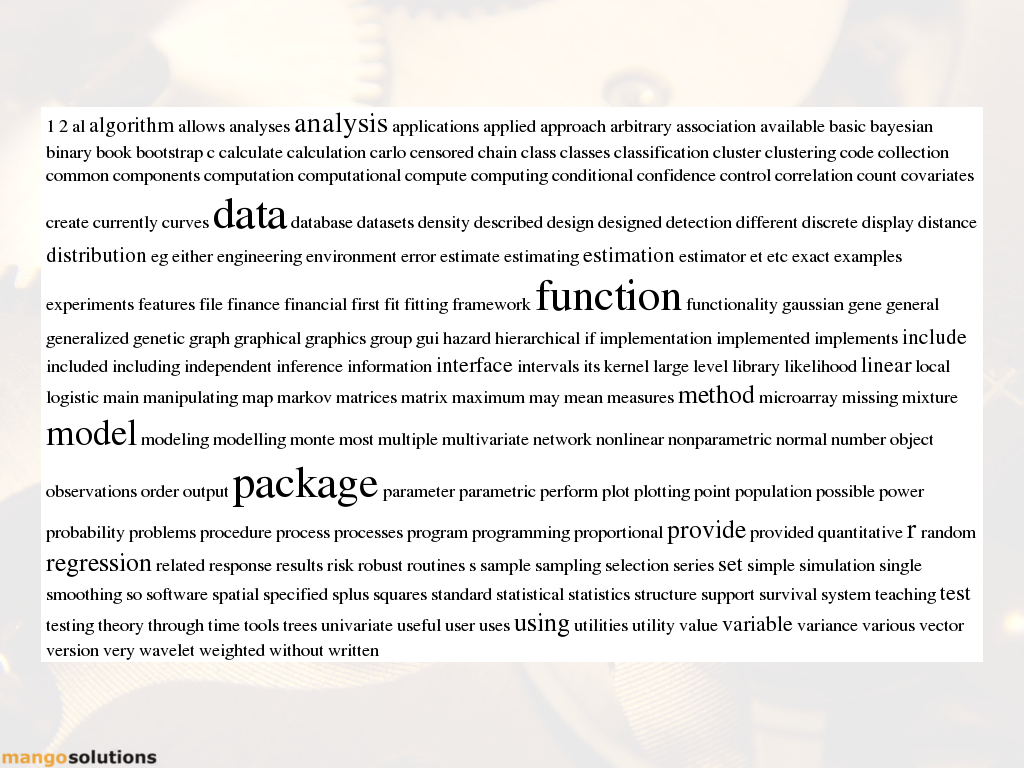
\includegraphics[width=\paperwidth]{pictures/tags2.png}} 
 \setbeamertemplate{navigation symbols}{}
 \begin{frame}[fragile][plain]
 \end{frame}
}



\begin{frame}[fragile][plain]

\end{frame}
 
\section{References}

\begin{frame}[fragile]
\frametitle{References}

XML references from W3C: 
\begin{itemize}
 \item E4X: \url{http://www.w3schools.com/e4x/default.asp}
 \item RSS: \url{http://www.w3schools.com/rss/default.asp}
\end{itemize}

R References
\begin{itemize}
 \item \rfun{XML} ($\hat{\Omega}$). \url{http://www.omegahat.org/RSXML/}
 \item \rfun{brew}: \url{http://www.rforge.net/brew/}
 \item \rfun{operators}: \url{http://www.mango-solutions.com}
\end{itemize}

\end{frame}

{
 \usebackgroundtemplate{
\includegraphics[width=\paperwidth]{pictures/gears3.jpg}} 
 \setbeamertemplate{navigation symbols}{}
 \begin{frame}[fragile][plain]

\begin{Huge}\textcolor{white}{\sf \bfseries Questions ?}\end{Huge}

\begin{flushright}
 \begin{Large}
\textcolor{white}{\bfseries \ttfamily rfrancois@mango-solutions.com}  
 \end{Large}
\end{flushright}


 \end{frame}
}



\end{document}
